\documentclass[portrait,final,20pt,ra0]{sciposter}
%------------------------------------------------------------------------------
\usepackage{epsfig}
\usepackage{amsmath}
\usepackage{amssymb}
\usepackage{multicol}
\usepackage[english]{babel}
\usepackage[utf8]{inputenc} %para poner tildes sin cdigo latex
\usepackage[numbers,super,sort&compress,merge,mcite]{natbib}%
\usepackage{booktabs}
\usepackage[hidelinks]{hyperref}
\usepackage{a0size}
\usepackage{boxedminipage}
\usepackage{color}
\usepackage{graphicx}
\usepackage{tabularx}
\graphicspath{{figures/}}
\usepackage{ifthen}
\usepackage{lettrine}
\usepackage{shadow}
\usepackage{times}
\usepackage{caption}
\usepackage{eso-pic}
\usepackage{transparent}
\usepackage{exscale}
\usepackage{pgfplots}
\pgfplotsset{compat=1.18} % o una versión cercana compatible
\usepackage{mathastext}
\usepackage{svg}
%------------------------------------------------------------------------------
\definecolor{BoxCol}{rgb}{0.038,0.038,0.351}
\definecolor{SectionCol}{rgb}{1.000,1.000,1.000}
\definecolor{mainCol}{rgb}{1.000,1.000,1.000}
\definecolor{TextCol}{rgb}{0.000,0.000,0.000}
\def\columnseprulecolor{\color{BoxCol}}
\renewcommand{\titlesize}{\Huge}
\renewcommand{\authorsize}{\LARGE}
\renewcommand{\instsize}{\large}
\setmargins[2.0cm]
\setlength{\parindent}{0.25cm}
\setlength{\parskip}{0.25cm}
\setlength{\columnsep}{2.0cm}
\setlength{\columnseprule}{0.14cm}
%------------------------------------------------------------------------------
\renewcommand{\labelitemi}{$\bullet$}
%------------------------------------------------------------------------------
\leftlogo[0.70]{ucsm}
\rightlogo[1]{Unimontes}
\title{Molecular dynamics interaction study on natural DPP4-inhibitors} 
\author{Stacanelli Camporioni, Isabela \textsuperscript{1}; Ponze Bellido, Leonardo\textsuperscript{2};Gomez Valdez, Badhin*.}
\institute{\textsuperscript{1}State University of Montes Claros, \textsuperscript{2}Catholic University of Santa Maria}
\email{\textsuperscript{1}isabelacamporioni@hotmail.com, \textsuperscript{2}leonardo.ponze.bellido@gmail.com} 
\conference{Centro de Investigación en Ingeniería Molecular, 05-30 enero, Arequipa, Perú.}
%------------------------------------------------------------------------------
\begin{document}
%------------------------------------------------------------------------------
%\AddToShipoutPictureBG*{\AtPageCenter{\transparent{0.2} \includegraphics[height=\paperheight]{DPP4-Comparison.png}}}
\AddToShipoutPictureBG*{%
  \put(\LenToUnit{\dimexpr\paperwidth/2},\LenToUnit{\dimexpr\paperheight/2}){%coloca en la mitad de la pagina
    \makebox(400,100){%x,y el centro de la imagen en el centro de la pagina
      \transparent{0.2}%transparencia
      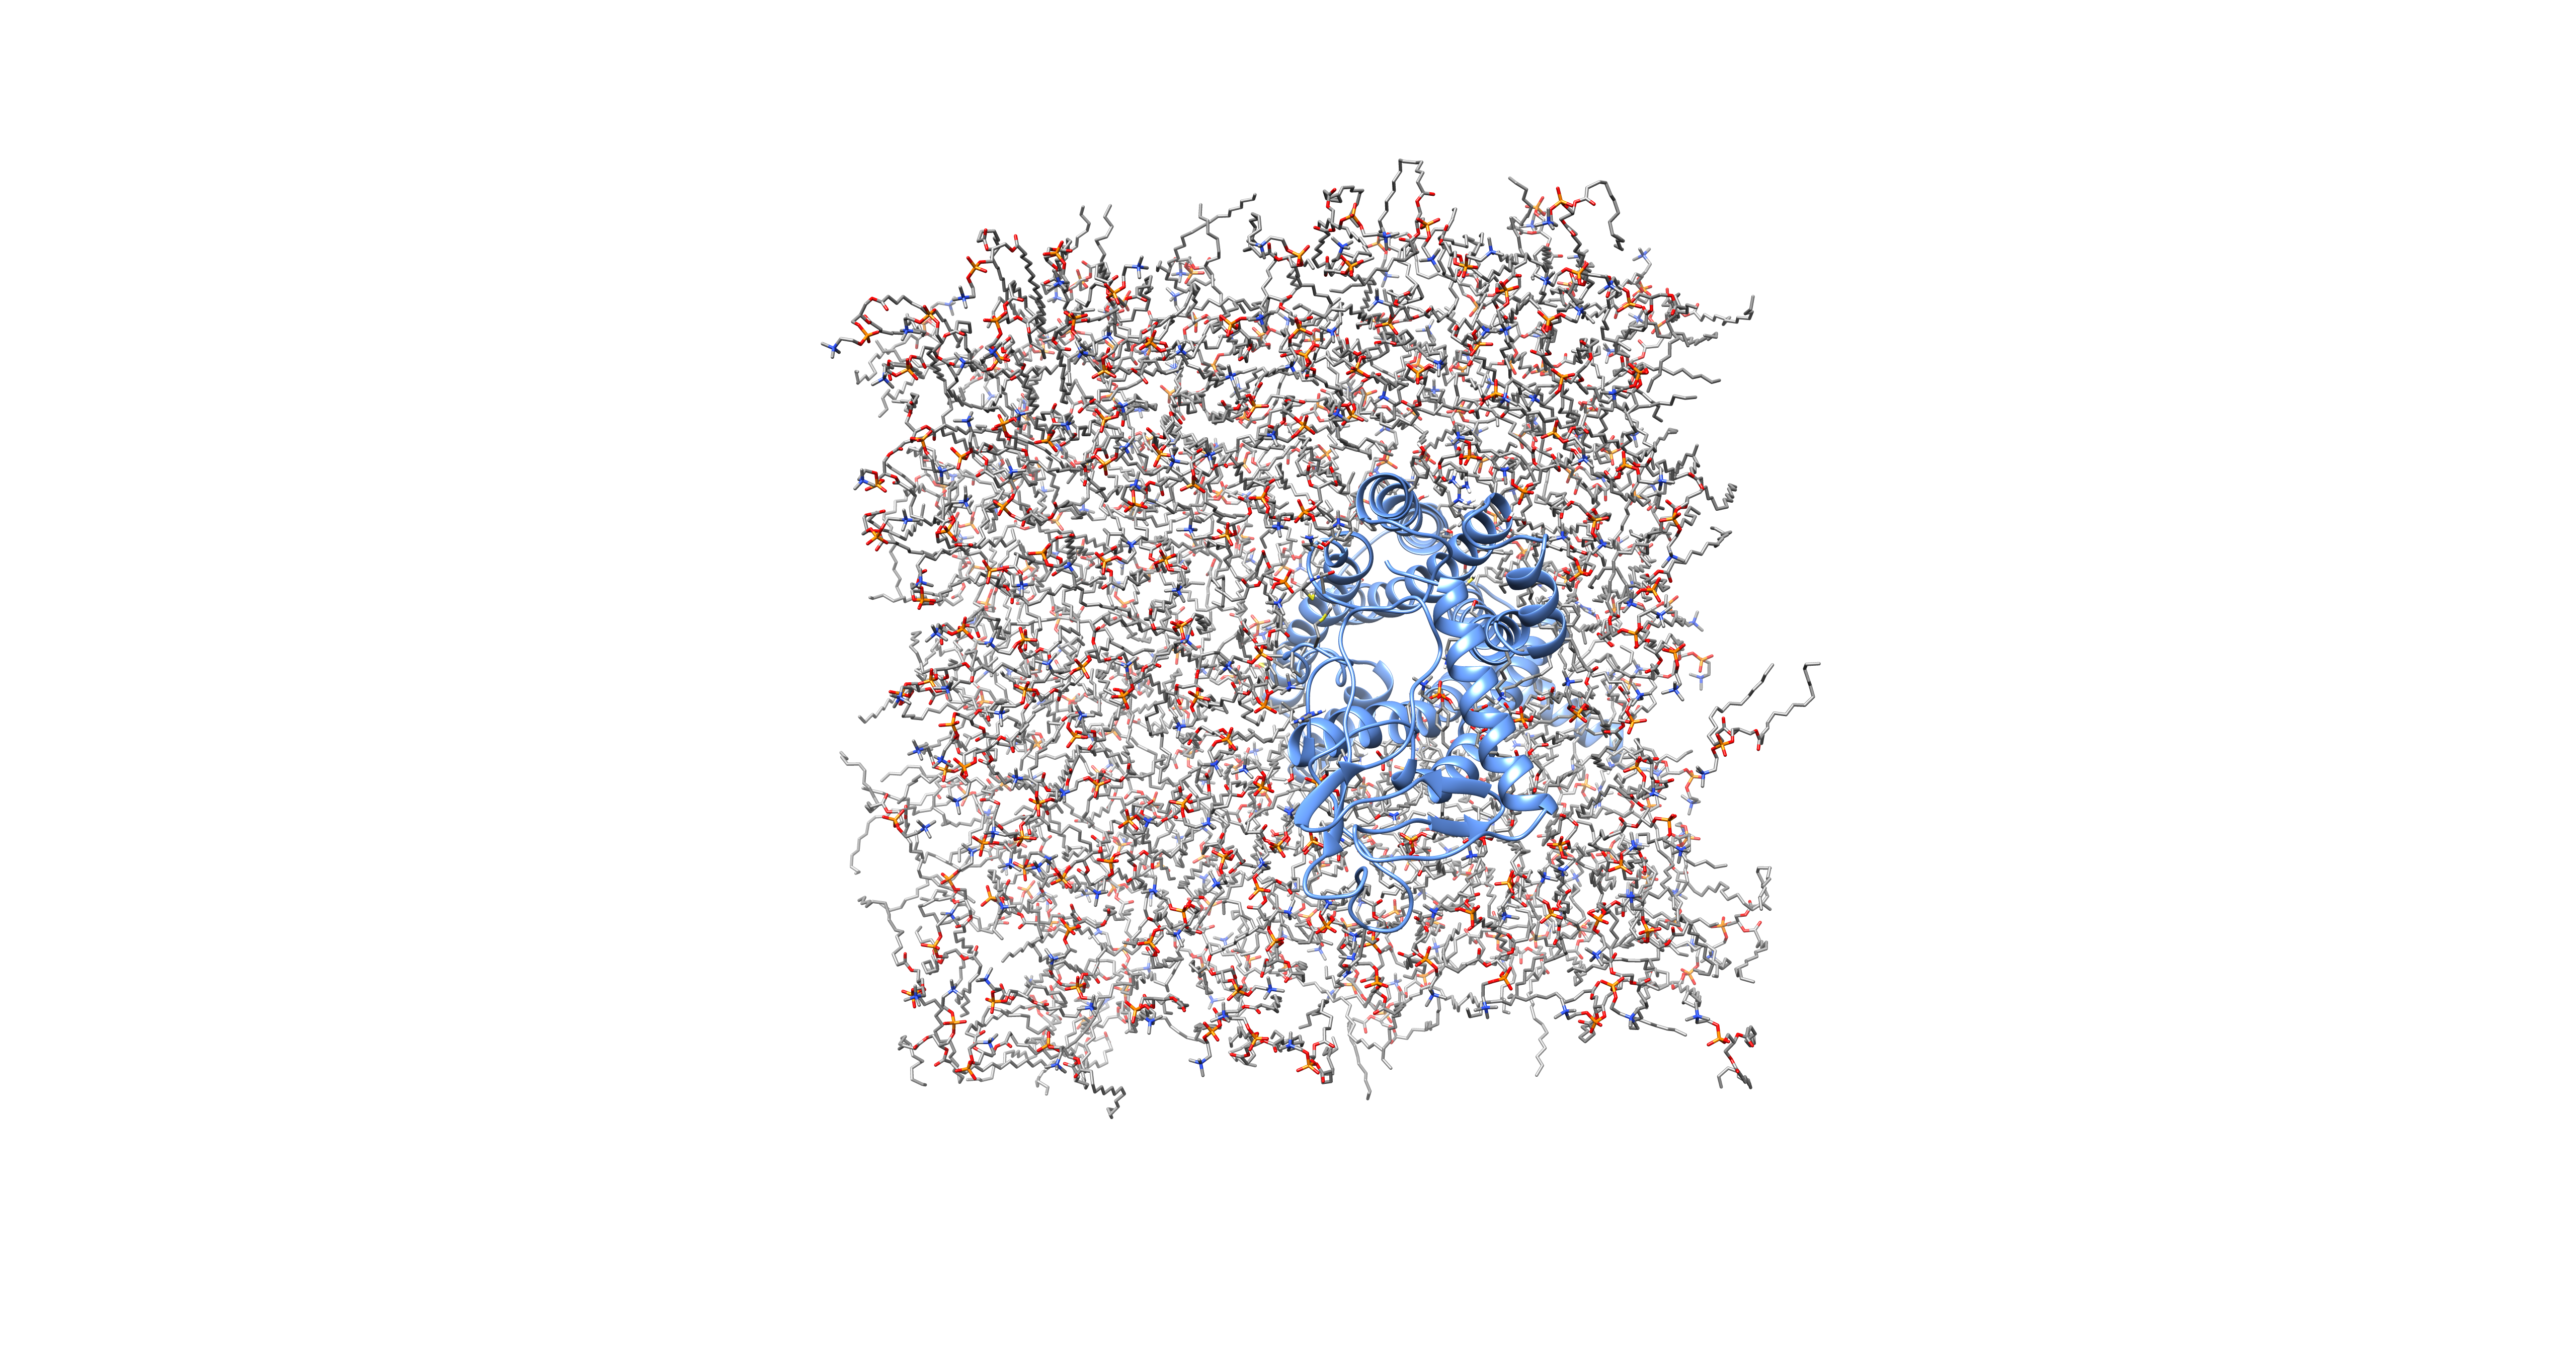
\includegraphics[height=1.2\paperheight,keepaspectratio]{image.png}%
    }%
  }%
}
%------------------------------------------------------------------------------
\maketitle{}
%------------------------------------------------------------------------------
\begin{multicols*}{3}
  %------------------------------------------------------------------------------
  \begin{abstract}
Diabetes mellitus is one of the human diseases with the highest morbidity and mortality rate in the world, being of the utmost importance to find alternative treatments to manage the complications of the disorder. DPP4 inhibitors prevent the degradation of GLP-1, thereby enhancing insulin secretion and compensating for insulin deficiency. In this article, through molecular engineering, we are able to analyse the binding afinity of potential natural DPP4 inhibitors by dynamic interactions and their ADMET toxicity profiles of the ligands as potential DPP4 inhibitors. In our study, twenty two compounds were selected for blind docking simulations, the five best-ranked binding ligands proceded with subsequent molecular dynamics simulations.  
  \end{abstract}
  %------------------------------------------------------------------------------
  \section*{Introduction}
Diabetes mellitus is a chronic metabolic disorder characterized by persistent hyperglycemia resulting from insulin resistance or defects in insulin secretion and/or action, and it is associated with high morbidity, mortality, and a substantial global economic burden \cite{Zarei_2024,2025}. Dipeptidyl Peptidase-4 (DPP-4) inhibitors are known for their ability to \cite{Shao2024, Hossain2024, Kuthati2025} prolong the activity of glucagon-like peptide-1 (GLP-1), thereby enhancing insulin secretion and reducing glucagon release \cite{Shao2024,Hossain2024, Kuthati2025}. In general, GLP-1RAs are preferred over DPP-4 inhibitors because they provide greater reductions in HbA1c and induce clinically meaningful weight loss, as demonstrated in clinical trials. In contrast, DPP-4 inhibitors produce only modest increases in endogenous GLP-1 levels, resulting in smaller glycemic improvements and minimal effects on body weight \cite{Gilbert2020}. In this context, DPP-4 \cite{Abbas2024} have gained increasing attention due to their role in glucose homeostasis and the development of novel pharmacological strategies \cite{Zarei_2024, Pezzoli2025}. In this study, we aim to identify natural compounds that can act as DPP-4 inhibitors using molecular engineering techniques, employing molecular modeling and docking approaches to screen for natural compounds that may interact with DPP-4, predicting their binding affinities and potential effects. This approach aims to discover low-cost, natural alternatives for diabetes treatment, offering new therapeutic options for managing the disease and its complications. 

%Diabetes mellitus is a chronic metabolic disorder characterized by persistent hyperglycemia resulting from insulin resistance, defects in insulin secretion, and/or action. This condition is associated with high morbidity and mortality rates, generating a substantial economic burden for global health systems (ZAREI et al., 2024; RAMANAND et al., 2025). Given this scenario, the search for effective therapies that act on glycemic homeostasis remains a priority in biomedical research. One of the consolidated therapeutic classes involves the incretin system. Dipeptidyl Peptidase-4 (DPP-4) inhibitors stand out for their ability to prolong the half-life and activity of glucagon-like peptide-1 (GLP-1). This mechanism results in the potentiation of glucose-dependent insulin secretion and the concomitant reduction of glucagon release (SHAO; ZHAO; SUN, 2024; HOSSAIN et al., 2024; KUTHATI; DAVULURI; WONG, 2025).In the current pharmacological landscape, GLP-1 receptor agonists (GLP-1RAs) are often preferred over DPP-4 inhibitors in certain clinical profiles, as they promote more significant reductions in glycated hemoglobin (HbA1c) and induce clinically meaningful weight loss, as demonstrated in various clinical trials (BROWN et al., 2021). In contrast, DPP-4 inhibitors tend to produce more modest increases in endogenous GLP-1 levels, resulting in smaller glycemic improvements and neutral effects on body weight (GILBERT; PRATLEY, 2020).Despite these comparative limitations, DPP-4 inhibitors maintain a relevant role and have received increasing attention. Their importance lies not only in maintaining glucose homeostasis but also in the potential development of novel pharmacological strategies targeting complementary pathways or differentiated safety profiles (ABBAS et al., 2025; PEZZOLI et al., 2025). Furthermore, the investigation of natural inhibitors emerges as a promising frontier, given the need for more accessible therapeutic alternatives with fewer adverse effects.In this context, the present study aims to identify natural compounds with inhibitory potential on DPP-4, utilizing molecular engineering techniques. Through molecular modeling and docking approaches, we seek to screen bioactive molecules capable of interacting with the enzyme's active site, predicting their binding affinities and potential pharmacodynamic effects. This approach aims to discover natural, low-cost alternatives for diabetes treatment, offering new therapeutic options for disease management and the mitigation of its chronic complications.

%ABBAS, G. et al. Dipeptidyl peptidase IV inhibitors as a potential target for diabetes: patent review 2019 – present. Expert Opinion on Therapeutic Patents, v. 35, n. 3, p. 239–250, 2025.

%BROWN, E. et al. SGLT2 inhibitors and GLP-1 receptor agonists: established and emerging indications. The Lancet, v. 398, n. 10296, p. 262-276, 2021.

%GILBERT, M. P.; PRATLEY, R. E. GLP-1 Analogs and DPP-4 Inhibitors in Type 2 Diabetes Therapy: Review of Head-to-Head Clinical Trials. Frontiers in Endocrinology, Lausanne, v. 11, p. 178, 2020.

%HOSSAIN, A. et al. Characterization of Plant-Derived Natural Inhibitors of Dipeptidyl Peptidase-4 as Potential Antidiabetic Agents: A Computational Study. Pharmaceutics, v. 16, n. 4, p. 483, 2024.

%KUTHATI, Y.; DAVULURI, V. N. G.; WONG, C. S. Therapeutic Effects of GLP-1 Receptor Agonists and DPP-4 Inhibitors in Neuropathic Pain: Mechanisms and Clinical Implications. Biomolecules, v. 15, n. 5, p. 622, 2025.

%PEZZOLI, A. et al. The Management of Cardiometabolic Risk in MAFLD: Therapeutic Strategies to Modulate Deranged Metabolism and Cholesterol Levels. Medicina, Kaunas, v. 61, n. 3, p. 387, 2025.

%RAMANAND, - et al. The Emergence of Bioactive Peptides as Anti-diabetic Agents: A Review. Current Protein & Peptide Science, v. 26, 2025.

%SHAO, D. W.; ZHAO, L. J.; SUN, J. F. Synthesis and clinical application of representative small-molecule dipeptidyl Peptidase-4 (DPP-4) inhibitors for the treatment of type 2 diabetes mellitus (T2DM). European Journal of Medicinal Chemistry, v. 272, p. 116464, 2024.

%ZAREI, M. et al. Incretin-based therapy: a new horizon in diabetes management. Journal of Diabetes & Metabolic Disorders, v. 23, n. 2, p. 1665-1686, 2024.

%GLP-1 is an incretin hormone secreted by enteroendocrine L-cells in the distal small intestine and colon, where it activates GLP-1 receptors. Physiologically, GLP-1 enhances glucose-dependent insulin secretion and suppresses glucagon release, thereby contributing to glycemic control\cite{Brown2021,Kuthati2025}.
%therapeutic targets such as GLP-1 \cite{Fang2024} and 


\begin{figure}
  \centering
  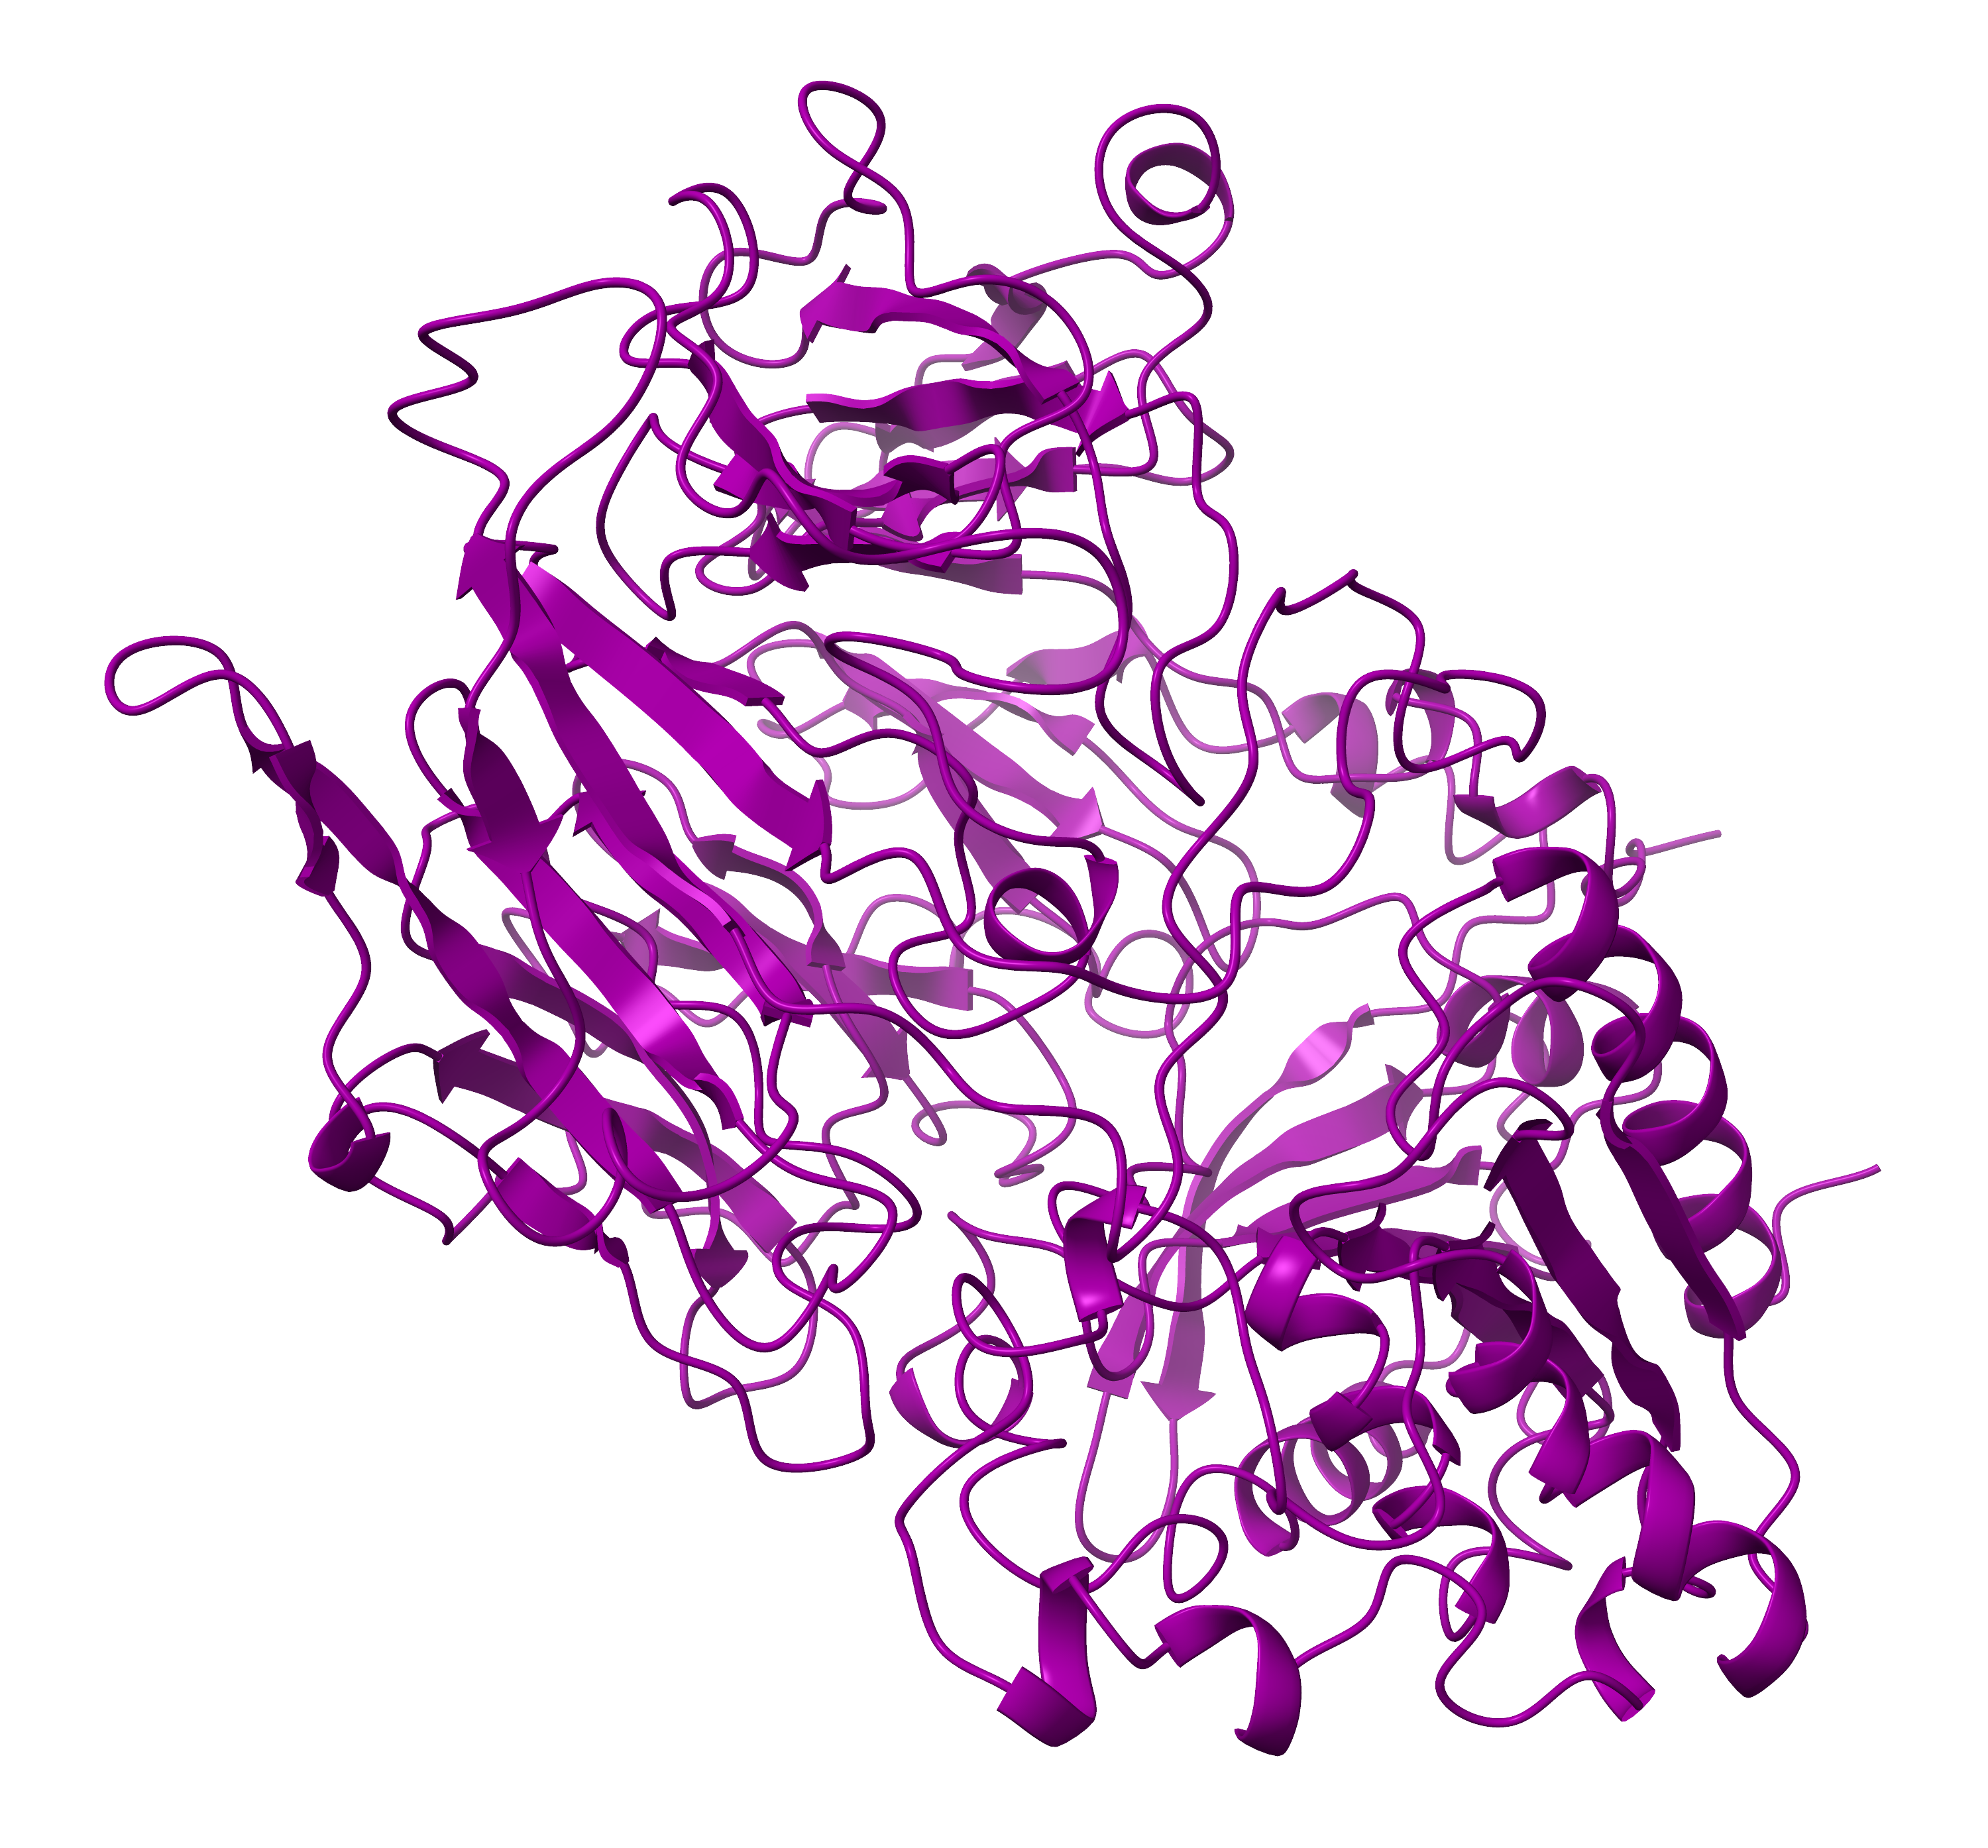
\includegraphics[width=0.9\textwidth]{DPP4.png}
  \captionof{figure}{Final DPP4 structure.}
  \label{fig-dpp4}
\end{figure}

  \section*{Methodology}
The present study focuses on several platforms and software tools, including the Protein Data Bank (PDB), Chimera, GROMACS, Gaussian. The DPP4 and GLP-1 protein structures had already been analyzed using ChimeraX and GROMACS software. A search for known natural ligands resulted in a total of 52 candidate compounds. SMILES notation and three-dimensional structures of the ligands were retrieved and verified through PubChem, Lotus, and Coconut databases. In the research,  twenty two natural potential DPP4 inhibitors were selected. The ligands were previously prepared through structural cleaning and geometric optimization using the Gaussian 16 software. The optimized ligands were converted to the PDBQT format for molecular docking. During this step, polar hydrogens were added and nonpolar hydrogens were merged according to AutoDock Vina requirements. Docking simulations were then performed using AutoDock Vina, generating 30 binding poses per ligand with a maximum of 1000 steps per run. The 5 best-ranked binding ligands were selected based on binding affinity scores from the DPP4 ligands (isoquercitrin (L1), rutin (L2), a-muurolene (L3), marmesinin (L4) and a flavone derivative (L5)), with values between -10.031 to -8.209 kcal/mol, which shows they had a good binding potential.

%https://www.microbiochemjournal.com/articles/ijcmbt-aid1008.pdf > A threshold of –5.5 kcal/mol (binding affinity) was set for the ligand-protein complexes for screening the effectively docked phytochemical. the highest affinity in experimentally validated inhibitors was-6.3 kcal/mol. This was set as threshold to screen potent and novel inhibitors from the set of phytochemicals, selected in this study.\textbf{} Kalhotra et al. (2018/2023) ou estudos similares em Frontiers in Pharmacology.

These selected complexes were further processed in Chimera, where hydrogens were added to the ligands to ensure proper protonation. Ligand topologies and parameters were then generated using the LigParGen server, which provided OPLS-compatible force field parameters, including ligand topology files (.itp), and structure files (.gro), for subsequent molecular dynamics simulations. Hirshfeld atomic charges were calculated for the ligands using Gaussian 16. The resulting charges were adjusted to ensure overall charge neutrality of each ligand and were subsequently incorporated into the ligand topology files for molecular dynamics simulations. After that, molecular dynamics simulations were carried out using GROMACS. The systems were subjected to energy minimization, followed by equilibration under NVT and NPT ensembles, and then to steered molecular dynamics (SMD) simulations. RMSD and RMSF analyses were performed on the GROMACS trajectories to evaluate the global stability and residue-wise flexibility of the protein–ligand complexes. Binding free energy calculations were then conducted using the Molecular Mechanics Poisson-Boltzmann Surface Area (MM/PBSA) method based on simulation snapshots to obtain refined binding affinity estimates beyond static docking performed in gmx\_MMPBSA. \newline\newline Figure \ref{fig-dpp4} shows the final stable state of the DPP4.

%CGENFF
%charm guii > force field, for lipids ---> gromacs
%RMSD and RMSF analyses were performed on the GROMACS trajectories to evaluate the global stability and residue-wise flexibility of the protein–ligand complexes. Binding free energy calculations were then conducted using the Molecular Mechanics Poisson-Boltzmann Surface Area (MM/PBSA) method based on simulation snapshots to obtain refined binding affinity estimates beyond static docking performed in gmx\_MMPBSA. These ligands were evaluated for toxicity using ADMET profiling. a proteina já esta minimizada, nvt, npt e sdm pelo gromacs;
%gaussian (clean, geometria), docking pelo pdbqt para cortar os hidrogenos por 30 modelos  em 1000 passos pela vina. selecionamos os 5 melhores com otimizacao hidrogewnos com quimera -- hidrogenio no ligante; com ligpargen fazemos a topologia dos ligantes (itp parametros ligantes e gro estrutura), os parametros dos atomos para fazer a simulacao em opls; usa gaussian 16 para cargas de hirsh field (calculo da orbita de cada atomo e faz o possivel para ser neutra, distribucao ), assim esta pronto pra simulacao, simulacao é com gromacs, fazemos os quatro parametros dnv --> rmsd (estabilizacao), rmsf faz a estabilizacao de cada proteina, o segundo resultado é  com mmpbsa > é um docking melhorado, conta todos os parametros pega a simulacao de gromacs e fazemos o calculo de afinidade final. top de proteinas)

%SYNTHETIC INHIBITORS; https://www.frontiersin.org/journals/molecular-biosciences/articles/10.3389/fmolb.2023.1130625/full
%https://acmcasereport.org/wp-content/uploads/2023/11/ACMCR-v11-2026.pdf

%"Para validar o protocolo de docking molecular e estabelecer um benchmark robusto de afinidade de ligação, selecionou-se um conjunto de 17 inibidores de DPP-4 (gliptinas), que representam o culminar de 17 anos de pesquisa e desenvolvimento (1998–2014) no tratamento do Diabetes Tipo 2. A escolha deste conjunto específico como controle positivo justifica-se por três fatores principais. Diversidade Estrutural e Química: As 17 gliptinas abrangem as principais classes químicas de inibidores da DPP-4, incluindo cianopirrolidinas (ex: Vildagliptina, Saxagliptina), xantinas (ex: Linagliptina), diprolil (ex: Teneligliptina) e pirimidinedionas (ex: Alogliptina). Essa variabilidade estrutural permite avaliar a capacidade do algoritmo de docking em predizer corretamente poses de ligação para diferentes esqueletos químicos ("scaffolds"), garantindo que o protocolo não seja enviesado para um único tipo de estrutura molecular. Modos de Ligação Caracterizados: Os mecanismos de interação destas gliptinas com o sítio ativo da DPP-4 estão bem documentados, envolvendo ocupações críticas nos bolsões S1, S2 e S2-extenso, bem como interações de ponte salina com os resíduos Glu205 e Glu206. A reprodução in silico destas interações conhecidas serve como validação essencial da acurácia do método, conforme sugerido por estratégias computacionais que utilizam fármacos aprovados (como a Saxagliptina) para comparar a eficácia de novos compostos. Relevância Clínica e Farmacológica: O grupo inclui tanto fármacos já aprovados por agências reguladoras (FDA/EMA) quanto compostos em fases avançadas de estudos clínicos, com valores de IC50​ experimentais conhecidos que variam na faixa nanomolar (ex: Sitagliptina IC50​=18 nM; Linagliptina IC50​=1.0 nM). Isso permite não apenas uma validação estrutural, mas também uma correlação comparativa de scores de energia livre de ligação com a potência biológica real.


\begin{figure}
  \centering
  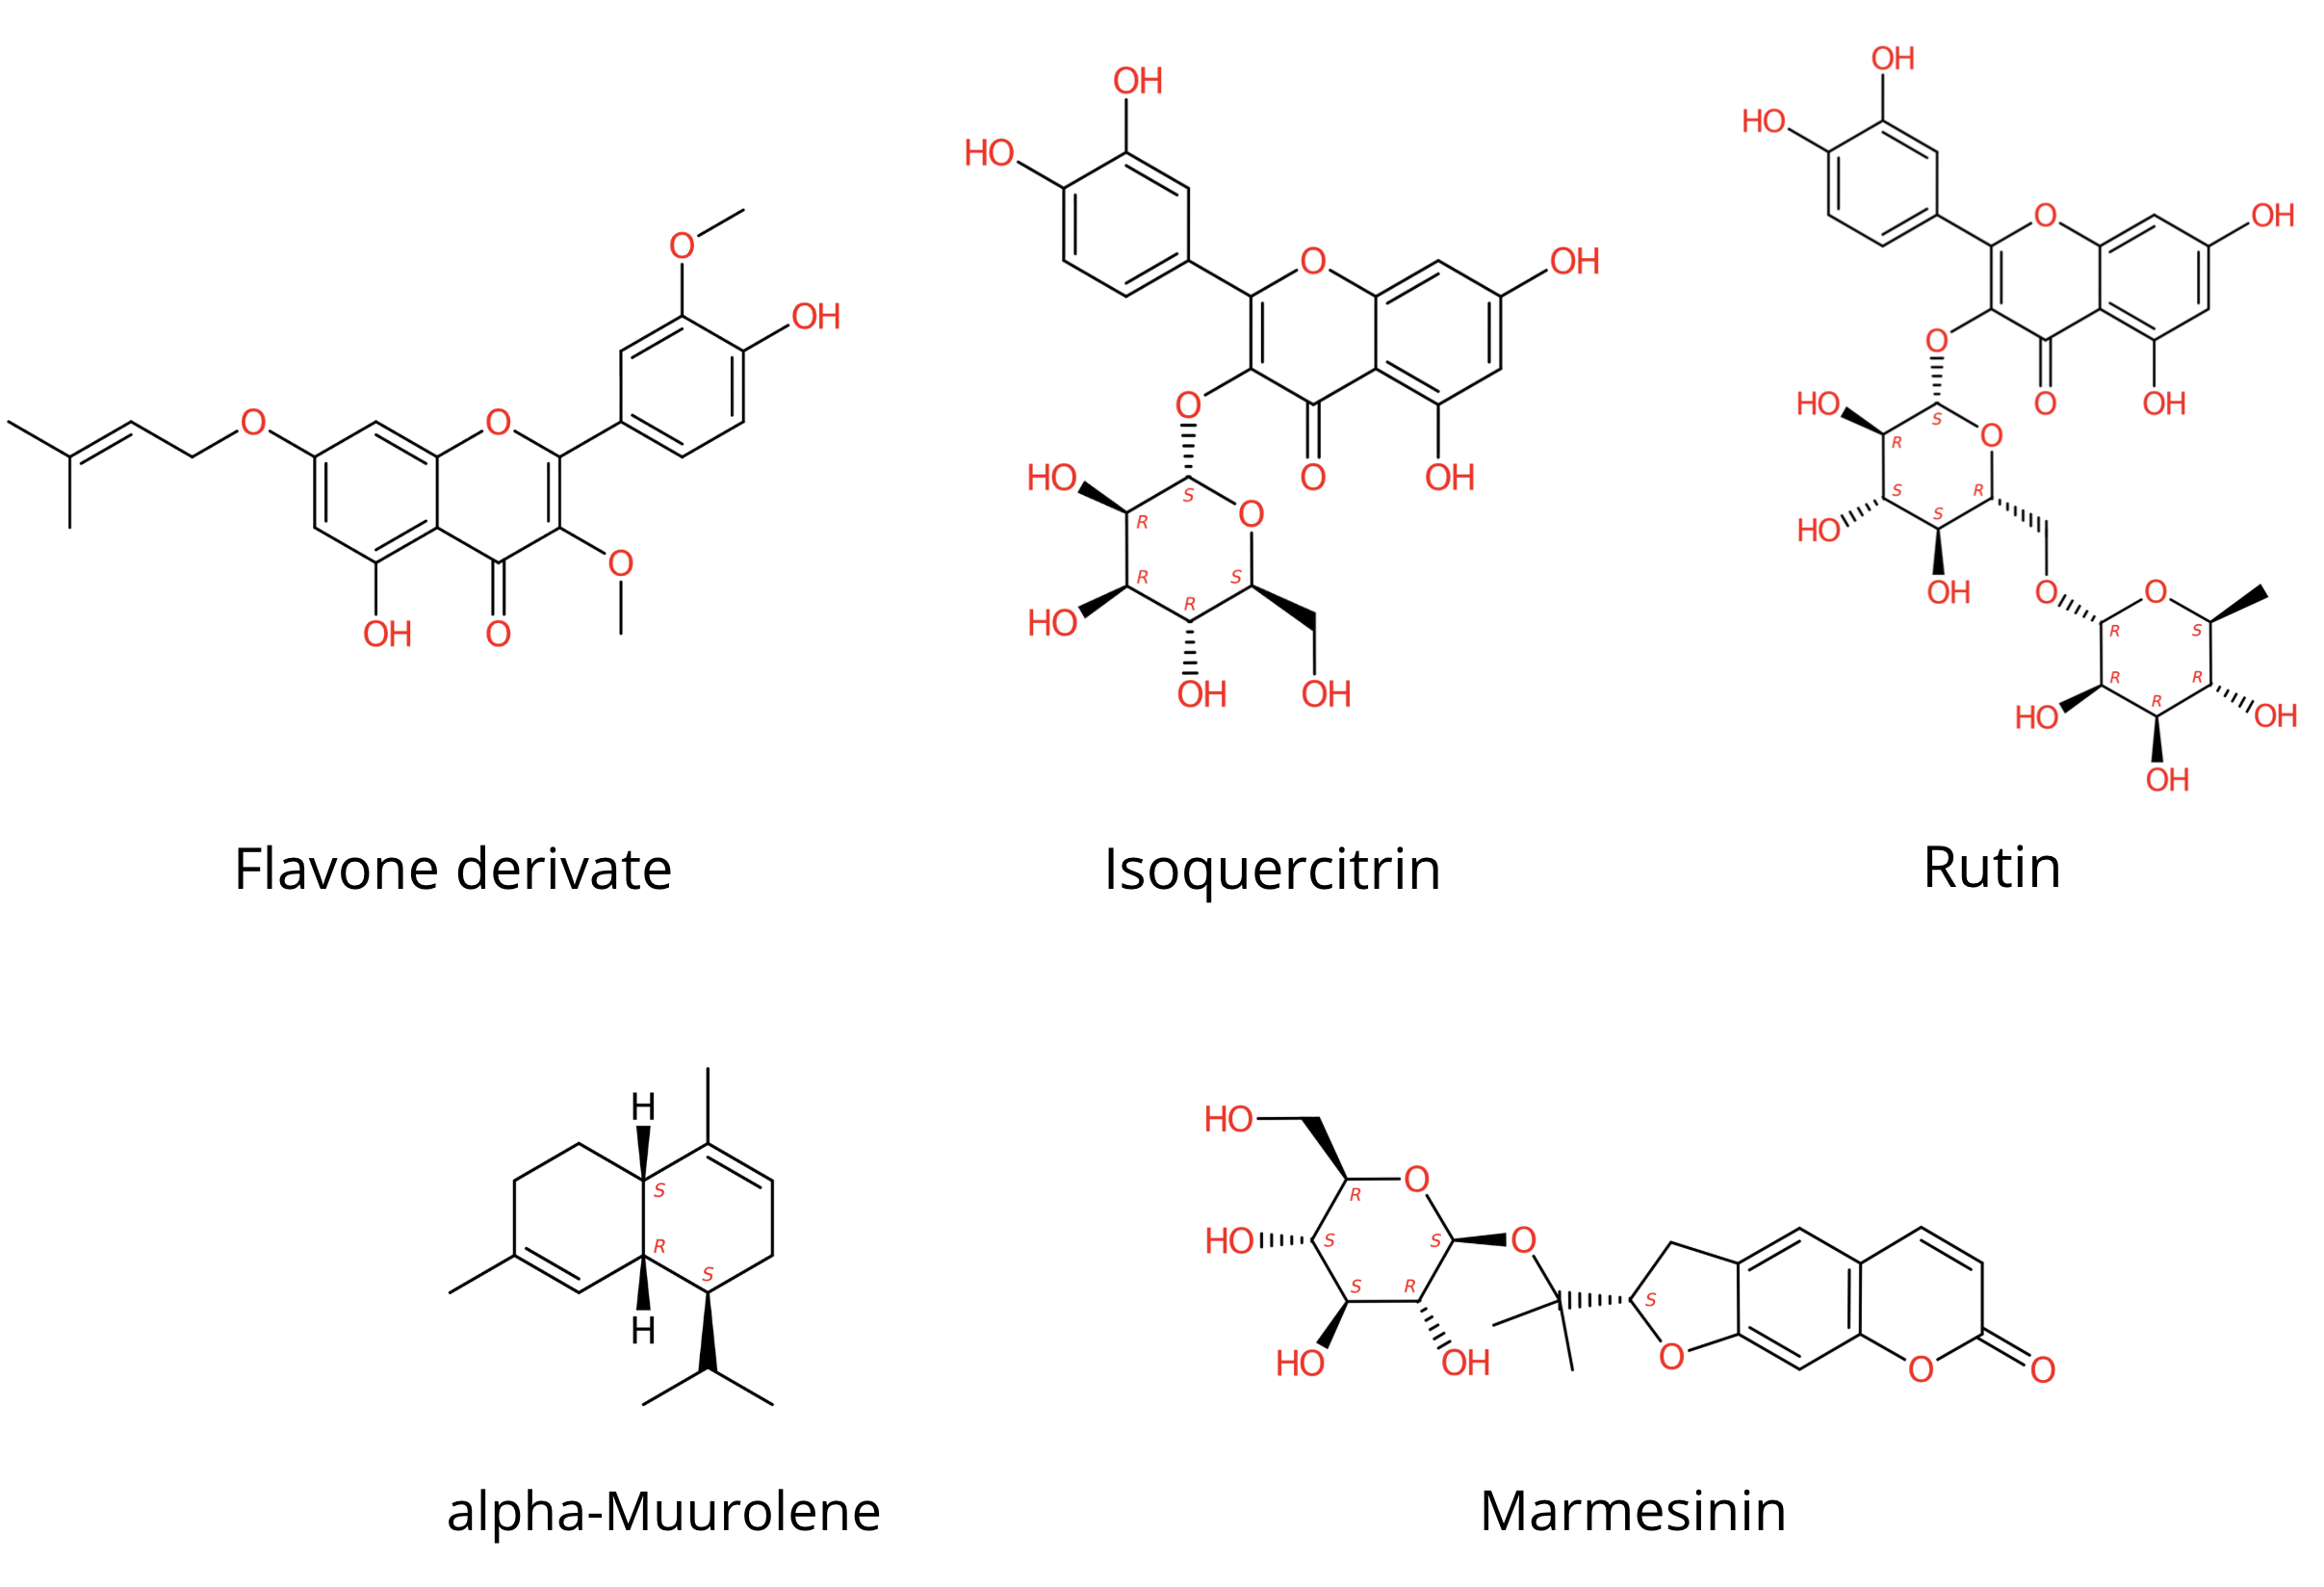
\includegraphics[width=0.8\textwidth]{Compounds.png}
  \captionof{figure}{Natural ligands selected for the molecular dynamics.}
  \label{fig-ligands}
\end{figure}
\\
\section*{Results and Discussion}


Figure \ref{fig:dpp4_pockets} shows the DPP4 pockets where the ligands bind.

\begin{figure}[htbp]
\centering
\includegraphics[width=1\columnwidth]{DPP4_DOCK.png}
\vspace{-1.0cm}
\captionof{figure}{DPP4 pockets.}
\label{fig:dpp4_pockets}
\end{figure}
\vspace{-1.0cm}

\vspace{0.0cm}
\begin{figure}[htbp]
\centering
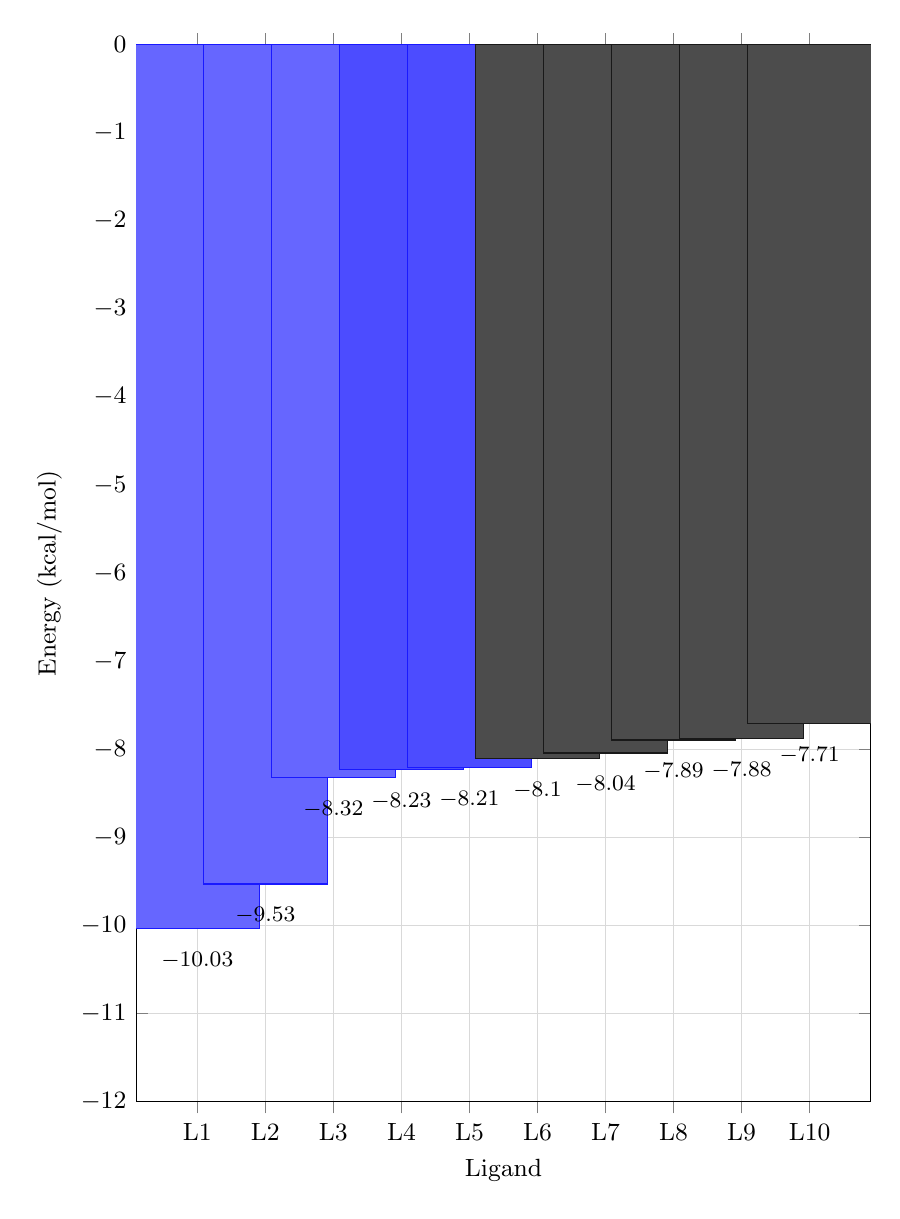
\begin{tikzpicture}
\begin{axis}[
    ybar,
    bar width=45pt,
    width=0.9\columnwidth,
    height=15cm,
    xlabel={Ligand},
    ylabel={Energy (kcal/mol)},
    ymin=-12, ymax=0,
    y dir=normal,
    symbolic x coords={L1, L2, L3, L4, L5, L6, L7, L8, L9, L10},
    xtick={L1, L2, L3, L4, L5, L6, L7, L8, L9, L10}, % <--- Aquí está el cambio    axis lines=box,
    grid=major,
    grid style={gray!30},
    tick label style={font=\small},
    label style={font=\small},
    yticklabel style={/pgf/number format/fixed},
    nodes near coords,
    nodes near coords style={black,font=\footnotesize, yshift=-5pt},
]

% Aquí cada barra con su color explícito:
\addplot+[bar shift=0pt, draw=blue!90, fill=blue!60] coordinates {(L1,-10.031)};
\addplot+[bar shift=0pt, draw=blue!90, fill=blue!60] coordinates {(L2,-9.530)};
\addplot+[bar shift=0pt, draw=blue!90, fill=blue!60] coordinates {(L3,-8.323)};
\addplot+[bar shift=0pt, draw=blue!90, fill=blue!70] coordinates {(L4,-8.227)};
\addplot+[bar shift=0pt, draw=blue!90, fill=blue!70] coordinates {(L5,-8.209)};
\addplot+[bar shift=0pt, draw=black!90, fill=black!70] coordinates {(L6,-8.101)};
\addplot+[bar shift=0pt, draw=black!90, fill=black!70] coordinates {(L7,-8.042)};
\addplot+[bar shift=0pt, draw=black!90, fill=black!70] coordinates {(L8,-7.894)};
\addplot+[bar shift=0pt, draw=black!90, fill=black!70] coordinates {(L9,-7.882)};
\addplot+[bar shift=0pt, draw=black!90, fill=black!70] coordinates {(L10,-7.711)};

\end{axis}
\end{tikzpicture}
\captionof{figure}{The 10 best results after blind docking.}
\label{fig:barplot}
\end{figure}
\vspace{-1.0cm}

%Blind docking simulations were performed using Vina, giving the best ligands and their binding poses. Following docking analysis, the five ligands with the most negative binding affinities (L1-L5) were selected for further study using Vina to predict their binding modes and affinities. The three-dimensional structures of these ligands were cross-checked against their PubChem counterparts, and hydrogens were added using ChimeraX. OPLS force field parameters for the two best ligands were generated using LigParGen, obtaining the necessary .gro and .itp files. Gaussian 16 software was employed to analyze the Hirshfeld charges of the three ligands, providing insight into electronic distribution to correct the ligand topology charges. 

Figure \ref{fig:barplot} shows the RMSD and RMSF of this equilibrium showing an excellent stable conformation. Figure \ref{fig:RMSD} shows that the stable state of the protein (RMSF).
During the RMSD and RMSF analysis, shown in Figure \ref{fig:RMSF} it was observed that L1 (isoquercitrin) destabilized the protein the most between 40 ns to 60ns. The other 4 ligands kept the protein in a fairly stable state. 

\vspace{-1.0cm}
\begin{figure}[htbp]
\centering 
\includegraphics[width=1\columnwidth]{figures/DPP4-multiplot-rmsd-best.pdf}
\vspace{0.3cm}
\vspace{-1.0cm}
\captionof{figure}{DPP4-ligands RMSD (top) and RMSF (bottom) after 100 ns.}
\label{fig:RMSD}
\end{figure}
\vspace{1.0cm}
\vspace{-1.0cm}
\begin{figure}[htbp]
\centering 
\includegraphics[width=1\columnwidth]{figures/DPP4-multiplot-rmsf-best.pdf}
\vspace{0.3cm}
\vspace{-1.0cm}
\captionof{figure}{DPP4-ligands RMSD (top) and RMSF (bottom) after 100 ns.}
\label{fig:RMSF}
\end{figure}
\vspace{1.0cm}

The reactivity of each ligand was analyzed and as shown in Figure \ref{fig:mmpbsa_stacked}. L5 (a flavone derivative) displayed the most negative energy out of all of them, meaning that it is the most reactive. L4 (marmesinin) had the second best reactivity, with a very small difference from L5.

\vspace{0.0cm}
% \begin{figure}[htbp]
% \centering
% \begin{tikzpicture}
% \begin{axis}[
%     ybar stacked,
%     bar width=95pt,
%     width=0.9\columnwidth,
%     height=30cm,
%     y dir=normal,
%     ymin=-75, ymax=25,
%     xlabel={Ligand},
%     ylabel={Energy (kcal/mol)},
%     symbolic x coords={L1, L2, L3, L4, L5},
%     xtick=data,
%     enlarge x limits=0.20, % <-- Esto reduce el espacio horizontal
%     x tick label style={font=\small},
%     y tick label style={font=\small},
%     legend style={
%         font=\scriptsize,
%         at={(0.8,0.95)},
%         anchor=north,
%         legend columns=2
%     },
%     grid=major,
%     grid style={gray!20},
%     axis lines=box,
%     nodes near coords,
%     nodes near coords style={black, font=\footnotesize},
% ]

% % \(\Delta\)VDWAALS
% \addplot+[draw=black!90, fill=red!70] coordinates {
%     (L1, -31.16)
%     (L2, -41.93)
%     (L3, -48.19)
%     (L4, -44.83)
%     (L5, -51.83)
    
% };

% % \(\Delta\)EEL
% \addplot+[draw=black!90, fill=violet!70] coordinates {
%     (L1, -3.67)
%     (L2, -5.83)
%     (L3, -3.59)
%     (L4, -0.32)
%     (L5, -3.52)
% };

% % \(\Delta\)EGB
% \addplot+[draw=black!90, fill=yellow!60!brown] coordinates {
%     (L1, 14.39)
%     (L2, 22.41)
%     (L3, 19.00)
%     (L4, 11.06)
%     (L5, 19.31)
% };

% % \(\Delta\)ESURF
% \addplot+[draw=black!90, fill=orange!70] coordinates {
%     (L1, -4.23)
%     (L2, -5.76)
%     (L3, -6.42)
%     (L4, -5.97)
%     (L5, -6.64) 
% };

% % Etiquetas del total arriba del gráfico
% \node[font=\small, anchor=south] at (axis cs:L1, -70) {\(\Delta E=-24.67\)};
% \node[font=\small, anchor=south] at (axis cs:L2, -70) {\(\Delta E=-31.11\)};
% \node[font=\small, anchor=south] at (axis cs:L3, -70) {\(\Delta E=-39.19\)};
% \node[font=\small, anchor=south] at (axis cs:L4, -70) {\(\Delta E=-40.07\)};
% \node[font=\small, anchor=south] at (axis cs:L5, -70) {\(\Delta E=-42.68\)};

% \legend{
%     \(\Delta\)VDWAALS,
%     \(\Delta\)EEL,
%     \(\Delta\)EGB,
%     \(\Delta\)ESURF
% }
% \end{axis}
% \end{tikzpicture}
% \captionof{figure}{Energy decomposition from MMPBSA for ligands L1-L5 bound to DPP4. Stacked bars represent contributions to total binding energy (\(\Delta\)Total).}
% \label{fig:mmpbsa_stacked}
% \end{figure} 
% \vspace{0.0cm}

\begin{figure}[htbp]
\centering 
\includegraphics[width=1\columnwidth]{figures/mmpbsa_stacked.pdf}
\captionof{figure}{DPP4-ligands MMPBSA energy decomposition.}
\label{fig:mmpbsa_stacked}
\end{figure}

\begin{table}
\begin{center}
\begin{tabular}{lrr}\toprule
Compound   &  $\Delta G_{\mathrm{bind}}$ \\\midrule
Flavone derivative (L5) &  -42.68\\ 
Marmesinin (L4) &  -40.07 \\
A-muurolene (L3) & -39.19  \\
Rutin (L2)      & -31.11 \\
Isoquercitrin (L1)      & -24.67 
\\\bottomrule
\end{tabular}
\end{center}
\end{table}

The toxicity profiles of the top five ligands were evaluated using in silico ADMET 3.0 analysis, revealing heterogeneous patterns. All compounds displayed high skin sensitization potential. Rutin (L2) emerged as the most toxic, showing strong hepatotoxic, mutagenic, and cytotoxic tendencies. Isoquercitrin also presented significant genotoxicity, while 5,4'-Dihydroxy-3,3'-dimethoxy-7-prenyloxyflavone (L5) exhibited moderate hepatotoxic and carcinogenic risks. $\alpha$-Muurolene (L3) showed a narrower toxicity profile, primarily affecting skin and eyes, whereas Marmesinin (L4) demonstrated considerable hepatotoxic and genotoxic potential. These findings suggest that the $\alpha$-Muurolene is the safest one based on the ADMET analysis.

%1. Rutin (L2)Among all evaluated ligands, Rutin (L2) exhibited the most severe and broad-spectrum toxicity profile, presenting substantial barriers to therapeutic applicability without optimization. Hepatotoxicity: The compound showed the highest probability of drug-induced liver injury (DILI) at 93.7%, highlighting a critical risk of hepatotoxicity. Genetic and Cellular Toxicity: Rutin demonstrated considerable risks for AMES mutagenicity (75.0%) and genotoxicity (86.8%). Additionally, cytotoxicity against A549 lung carcinoma cells was predicted at 86.0%.  Other Endpoints: The safety profile is further burdened by extremely high probabilities of skin sensitization (99.7%), eye irritation (90.0%), and ototoxicity (88.4%).

%2. Marmesinin Marmesinin demonstrated substantial toxicity, comparable in severity to Rutin, with a specific focus on hepatic and genetic endpoints.  Hepatotoxicity and Mutagenicity: The compound displayed a very high probability of DILI (92.8%) and the highest AMES mutagenicity among the group (90.9%). Systemic Risks: Safety concerns are further elevated by high predictions for skin sensitization (95.0%), genotoxicity (89.3%), and ototoxicity (85.5%), suggesting potential risks regarding genomic stability and liver function.

%3. Isoquercitrin Isoquercitrin showed a pronounced toxicity profile, primarily associated with genetic damage and dermatological risks. Genetic Toxicity: The compound presented a high probability of DNA mutation (75.1%) and notably elevated genotoxicity (92.1%). Cytotoxicity and Irritation: Like Rutin, Isoquercitrin showed a high probability of A549 cell cytotoxicity (86.0%), along with extremely high skin sensitization potential (99.5%) and substantial eye irritation risk (91.3%).

%4. 5,4′-Dihydroxy-3,3′-dimethoxy-7-prenyloxyflavone: This compound displayed a moderate-to-high toxicity profile affecting multiple organ systems, with specific concerns regarding long-term exposure.Systemic Toxicity: It showed a high likelihood of drug-induced liver injury (80.5%) and respiratory toxicity (80.3%).Carcinogenicity: Notably, this ligand was associated with carcinogenicity (70.6%), alongside severe eye irritation (93.0%) and skin sensitization (85.4%).

%5. α-Muurolene In contrast to the flavonoids and coumarins analyzed above, α-Muurolene exhibited a comparatively narrower and less systemic toxicity spectrum. Dermal and Ocular Focus: Its primary predicted adverse effects were restricted to contact surfaces, including eye corrosion (93.0%), eye irritation (95.0%), and skin sensitization (82.0%).Relative Systemic Safety: The absence of high probability predictions for hepatotoxicity, genotoxicity, or mutagenicity suggests that α-Muurolene may present a more limited systemic toxicity profile relative to the other ligands.


\section*{Conclusions}
This study evaluated the interaction of natural ligands with GLP-1, a key target in diabetes treatment. Following blind molecular docking, 5 potential candidates were chosen based on their binding energies and after molecular dynamics simulations it was revealed that 5,4'-Dihydroxy-3,3'-dimethoxy-7-prenyloxyflavone, a flavone derivative had the best reactivity with DPP4 and exhibited moderate hepatotoxic and carcinogenic risks, being the most promising candidate for further optimization. Marmesinin showed the second best reactivity, despite its high ADMET toxicity. Alfa-muurolene showed the third best reactivity, with the least toxicity profile, exibiting a good potential for further investigation. However, isoquercitrin and rutin, despite their good binding affinities, demonstrated significant toxicity risks, limiting their therapeutic potential. In conclusion, this study shows possible therapeutic candidates for DPP4 inhibition in diabetes treatment, integrating dynamic studies and toxicity profiling in selecting potential DPP4 inhibitors for diabetes treatment. Further experimental validation will be essential to confirm these findings. 


\section*{Acknowledgement}%{acknowledgement}
This study was conducted under the surveillance of Professor Badhin, in the computational laboratory of the Catholic University of Santa Maria. We would like to thank Professor Badhin for the hospitality and kindness, allowing the realization of the internship and to learn about molecular engineering, its importance, and the opportunity to grow in a enriching research environment. We are also grateful for the computational infrastructure that facilitated our analysis. We thank our tutors and colleagues for their patience invaluable guidance, feedback, and collaboration.  %------------------------------------------------------------------------------
  \bibliography{references}
  \bibliographystyle{JAmChemSoc}
  
%Zarei M, Sahebi Vaighan N, Farjoo MH, Talebi S, Zarei M. Incretin-based therapy: a new horizon in diabetes management. J Diabetes Metab Disord. 2024 Aug 17;23(2):1665-1686. doi: 10.1007/s40200-024-01479-3. PMID: 39610543; PMCID: PMC11599551.

%Ramanand -, Rohit Singh, Vedpal Singh, Archita Katrolia, The Emergence of Bioactive Peptides as Anti-diabetic Agents: A Review, Current Protein & Peptide Science; Volume 26, Issue , Year 2025, e13892037386831.

%Abbas, G., Akhtar, M. S., Haq, Q. M., Al Amri, I. S., Wang, D., & Hussain, H. (2025). Dipeptidyl peptidase IV inhibitors as a potential target for diabetes: patent review 2019 – present. Expert Opinion on Therapeutic Patents, 35(3), 239–250. https://doi.org/10.1080/13543776.2024.2446226

%Fang H, Niu B, Chen Q. The Discovery and Development of Glucagon-Like Peptide-1 Receptor Agonists. Curr Med Chem. 2024;31(20):2921-2943. doi: 10.2174/0929867330666230416153301. PMID: 37062063.

%Pezzoli A, Abenavoli L, Scarcella M, Rasetti C, Svegliati Baroni G, Tack J, Scarpellini E. The Management of Cardiometabolic Risk in MAFLD: Therapeutic Strategies to Modulate Deranged Metabolism and Cholesterol Levels. Medicina (Kaunas). 2025 Feb 23;61(3):387. doi: 10.3390/medicina61030387. PMID: 40142198; PMCID: PMC11944025.

%Shao DW, Zhao LJ, Sun JF. Synthesis and clinical application of representative small-molecule dipeptidyl Peptidase-4 (DPP-4) inhibitors for the treatment of type 2 diabetes mellitus (T2DM). Eur J Med Chem. 2024 Jun 5;272:116464. doi: 10.1016/j.ejmech.2024.116464. Epub 2024 May 1. PMID: 38704940.

%Hossain A, Rahman ME, Faruqe MO, Saif A, Suhi S, Zaman R, Hirad AH, Matin MN, Rabbee MF, Baek KH. Characterization of Plant-Derived Natural Inhibitors of Dipeptidyl Peptidase-4 as Potential Antidiabetic Agents: A Computational Study. Pharmaceutics. 2024 Apr 1;16(4):483. doi: 10.3390/pharmaceutics16040483. PMID: 38675143; PMCID: PMC11053753. 

%Brown E, Heerspink HJL, Cuthbertson DJ, Wilding JPH. SGLT2 inhibitors and GLP-1 receptor agonists: established and emerging indications. Lancet. 2021 Jul 17;398(10296):262-276. doi: 10.1016/S0140-6736(21)00536-5. Epub 2021 Jun 30. PMID: 34216571.

%Kuthati Y, Davuluri VNG, Wong CS. Therapeutic Effects of GLP-1 Receptor Agonists and DPP-4 Inhibitors in Neuropathic Pain: Mechanisms and Clinical Implications. Biomolecules. 2025 Apr 26;15(5):622. doi: 10.3390/biom15050622. PMID: 40427515; PMCID: PMC12108864. 

%Gilbert MP, Pratley RE. GLP-1 Analogs and DPP-4 Inhibitors in Type 2 Diabetes Therapy: Review of Head-to-Head Clinical Trials. Front Endocrinol (Lausanne). 2020 Apr 3;11:178. doi: 10.3389/fendo.2020.00178. PMID: 32308645; PMCID: PMC7145895.



  %------------------------------------------------------------------------------
\end{multicols*}
%------------------------------------------------------------------------------
\end{document}
